\section{Challenges of Text Entry in Virtual Reality}
Text entry is a  an extreme use in testing our ability to interact between the physical and virtual world.

\subsection{Latency}
Typing is complex interaction that requires a high-bandwidth feedback loop~\cite{McGill:2015:DRO:2702123.2702382}.
Latency is a barrier in achieving a seamless interaction between the real and virtual~\cite{leedesigning}.

In virtual reality, latency is the time between movement of the user's head and the updated image being displayed on the screen.  
This includes time includes the times for fusion, image transmission,
rendering, sensor response and display response.
This is commonly referred to as the \textit{motion-to-photon} latency.

To achieve a genuine sense of presence~\cite{schuemie2001research} in virtual reality, the total \textit{motion-to-photon} latency must be less than 20 milliseconds~\cite{jerald2009relating,jerald2010scene,bailey2004latency} for head movement.
Some existing systems have a latency as high as 80 milliseconds ~\cite{lincoln2016motion,dallaire2016animated}.

Touch-based interactions need even tighter tolerances on latency compared to head movement described above.
Research on touchscreens finds that for a user to perceive display elements as naturally being affected by touch, there is a perceptual floor between 2  and 11 milliseconds below which users do not notice lag~\cite{Jota:2013:FFE:2470654.2481317,Ng:2012:DLD:2380116.2380174}.

Further, they find that latencies down to 2.38 milliseconds are required to alleviate user perception when dragging~\cite{Jota:2013:FFE:2470654.2481317,Ng:2012:DLD:2380116.2380174}.

\subsection{Reduced Precision}
Haptic feedback and physical constraints in real world input devices help to define interactions. 
Fine-grained control is difficult in in virtual reality and restricts users to the coarse manipulation of virtual objects.
Input device that excluded the use of the fingers are slower~\cite{Zhai:1996:IMG:238386.238534}.

\subsection{Limited Proprioception}
Manipulation in virtual reality is difficult because users must do without the haptic contact with keyboard buttons they rely on in the real world to orient themselves.
To compensate for this, we propose using relative instead of absolute positioning for entry.


\section{Design Goals}
Before describing the prototypes and lessons learned, we present five high-level design goals that focus on input metrics, user experience, and adaptability.
These goals are informed by related work and our experience building other systems.

\subsection{Efficient}
How closely does the new device approach exceed the speed of the best devices for text input in virtual reality?

\subsection{Learnable}
How long does the device take to learn?
Does it rely on existing skills?
Is there ways for the user to transition from being a novice to an expert?

\subsection{Practical}
Is the input method usable today?
Moreover, will it be usable in the future given the where we think virtual reality controller are heading?

\subsection{General}
Is the text input method useful across multiple types of applications?
Can the user type their username, password, and a message to a friend?

\subsection{Usable}
Desktop user sessions are longer than mobile~\cite{Kamvar:2009:CIM:1526709.1526817}.
We hypothesize that virtual reality will have a user session time closer to that of a desktop computer than a mobile phone.
Once a user has take the time to wear the head mounted display and controller, the session will
Midair interactions are prone to fatigue and lead to a feeling
of heaviness in the upper limbs~\cite{Hincapie-Ramos:2014:CEM:2556288.2557130}, commonly known as the \textit{gorilla arm effect}.
Will the user be able to use the text input method comfortably?
Can they use it for as long as they use as they their computer at night?

\section{Prototyping Process}
During the prototyping process, we ask a users to type a few sentences using the input device. 
The users was given little to no instruction about how the input device worked.
The goals of this process was to explore the performance potential of each input device and to investigate if users could understand the visual interface.
We record how long the input took, their understanding of the input device, and their other feedback.

\subsection{Design \#1 - External Camera}
\vspace*{.1cm}

\includegraphics[width=.9\columnwidth]{figures/sigchi-logo}

For the first pilot, we build a prototype that streams from the front facing camera on the head mounted display into the virtual enviroment.
The camera is pointed at a soft mobile keyboard.
The goals of this pilot is to investigate how latency and presence, particular of the fingers, affect performance.
Latency is an inhibitor to fast input.
Additionally, muscle memory is not as accurate as we expect and drifts quickly after a few taps.

\subsection{Design \#2 - 26-key Tap}
\vspace*{.1cm}
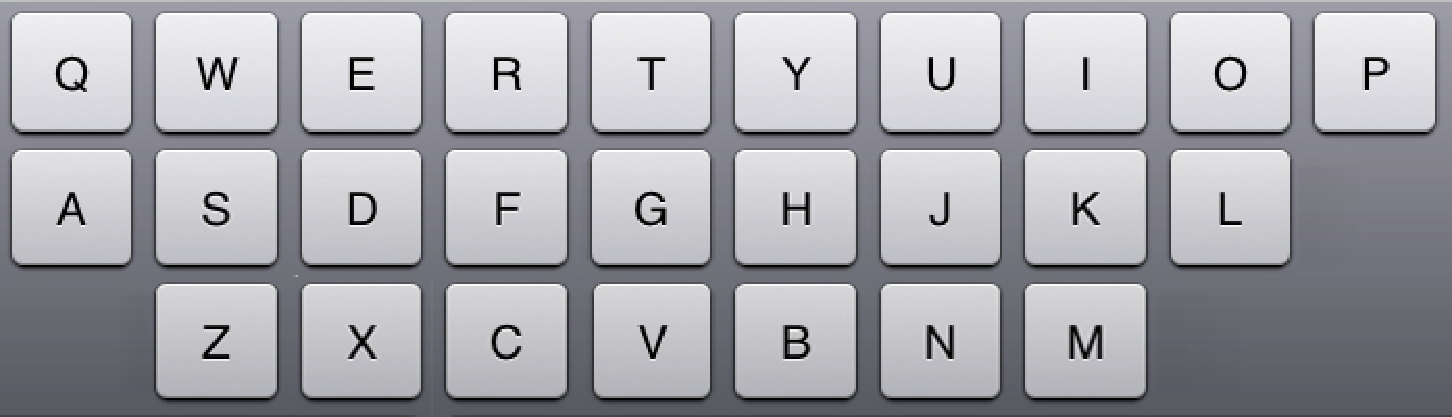
\includegraphics[width=.9\columnwidth]{figures/26Tap}

Layout and formatted exactly as regular mobile keyboard.
Aggressive autocorrect algorithm adjusted for typos and phonetic misspelling are applied.
The advantage of such keyboard is that the user does not need to change his interaction with a keyboard at all.
We noticed an unexpected phenomenon.
The user would  position their finger through gesture onto the desired key, but when they went to tap the key the lifting and lowering of the finger so that the proper key was not selected. 


\subsection{Design \#3 - 26-key Drag}
\vspace*{.1cm}
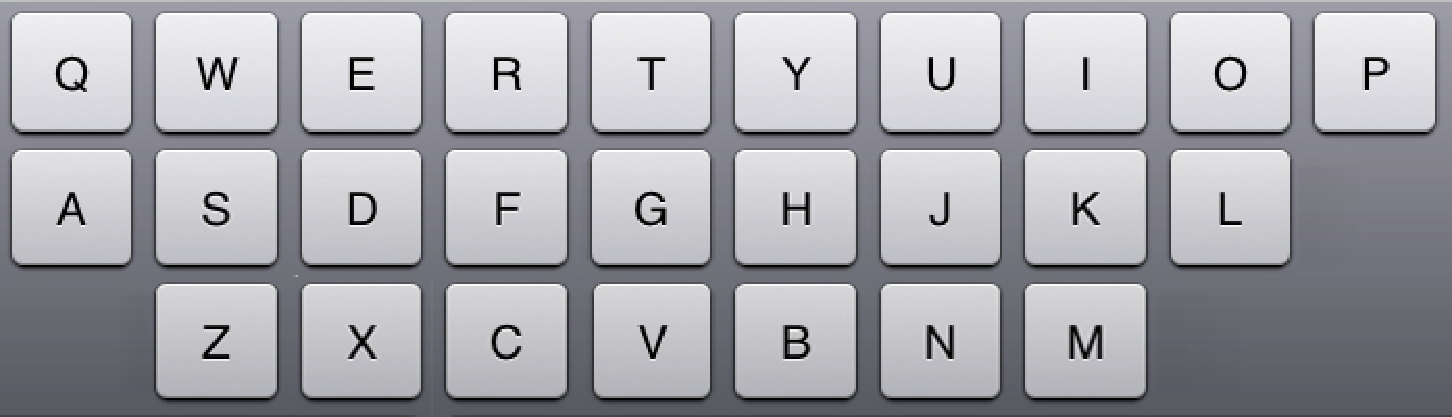
\includegraphics[width=.9\columnwidth]{figures/26Tap}

Similar to the 26-key tap, the layout of the mobile QWERTY keyboard is preserved, except tapping is replaced by dragging to specific keys.
Same autocorrect algorithm is applied


\subsection{Design \#4 - 8-key Drag}
\vspace*{.1cm}
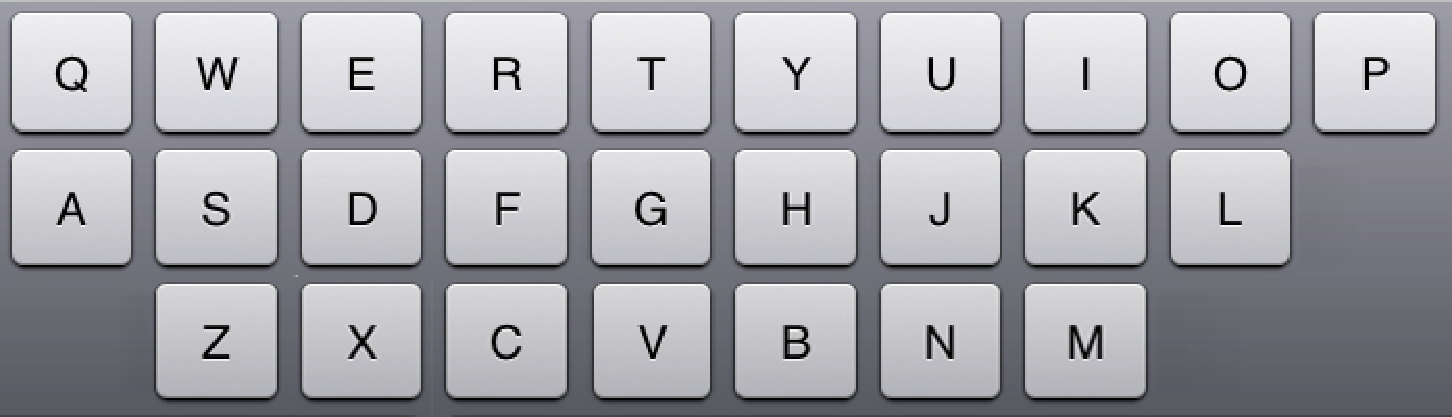
\includegraphics[width=.9\columnwidth]{figures/26Tap}

QWERTY keyboard is broken into 8 regions instead of 6.
User interact with this keyboard through dragging.
Both hands are required, with each hand dragging four directions (left, up, right, down) to input the 8 regions.

\subsection{Design \#5 - 6-key Tap}
\vspace*{.1cm}
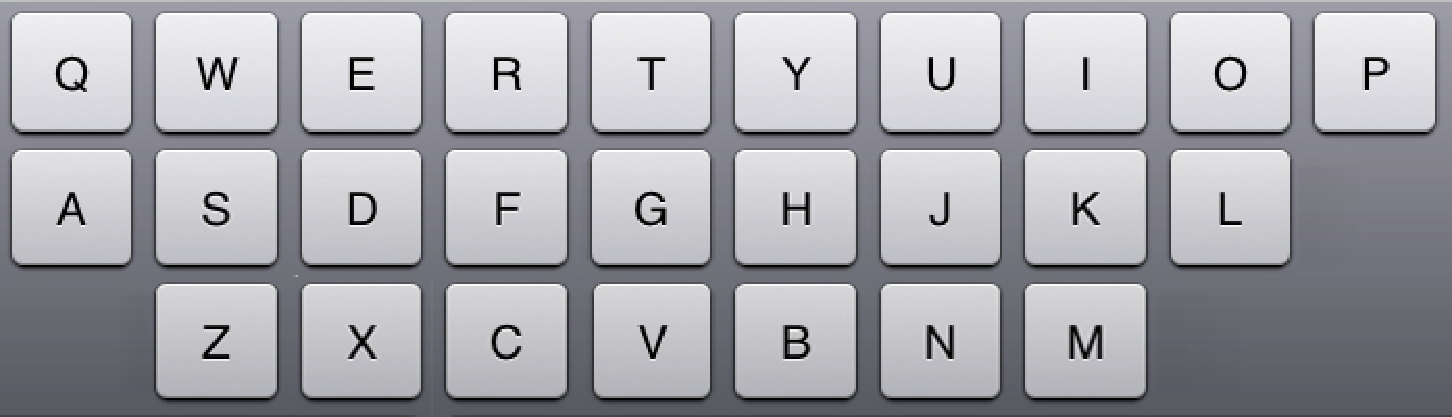
\includegraphics[width=.9\columnwidth]{figures/26Tap}

This is our first design utilizing batched keys. QWERTY keyboard is divided into 6 sections. Tapping corresponding regions triggers input for a whole section.
A word recommender algorithm in back end is required.


\subsection{Design \#6 - 6-key Drag}
\vspace*{.1cm}
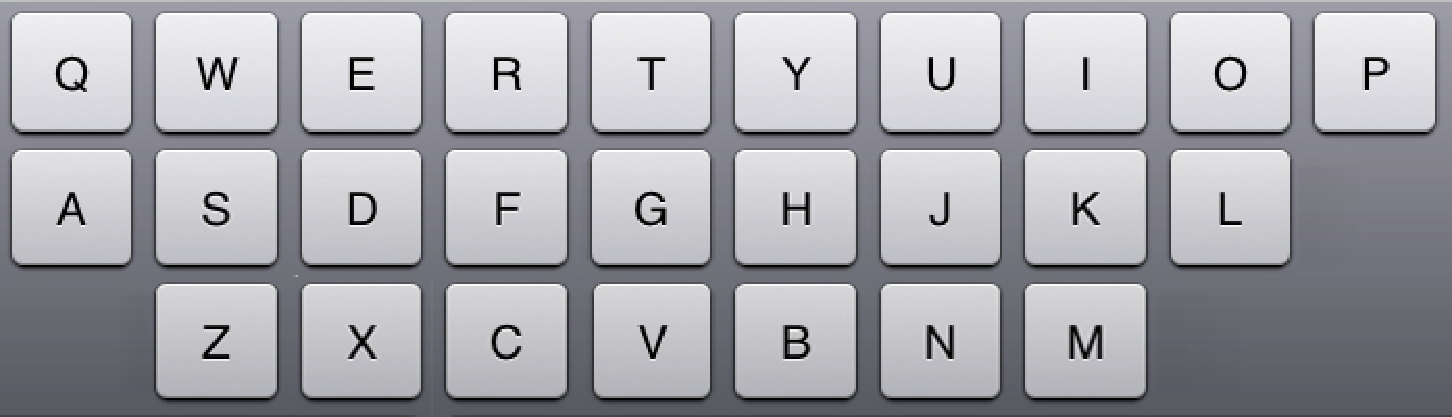
\includegraphics[width=.9\columnwidth]{figures/26Tap}

Similar to 6 keys tap, the method of interaction is changed to drag instead of tap.
A word recommender algorithm in back end is required.


